
	\subsubsection{Back-end}
	\paragraph{Informazioni sul package} 
		\begin{figure}[H] 
			\begin{center} 
				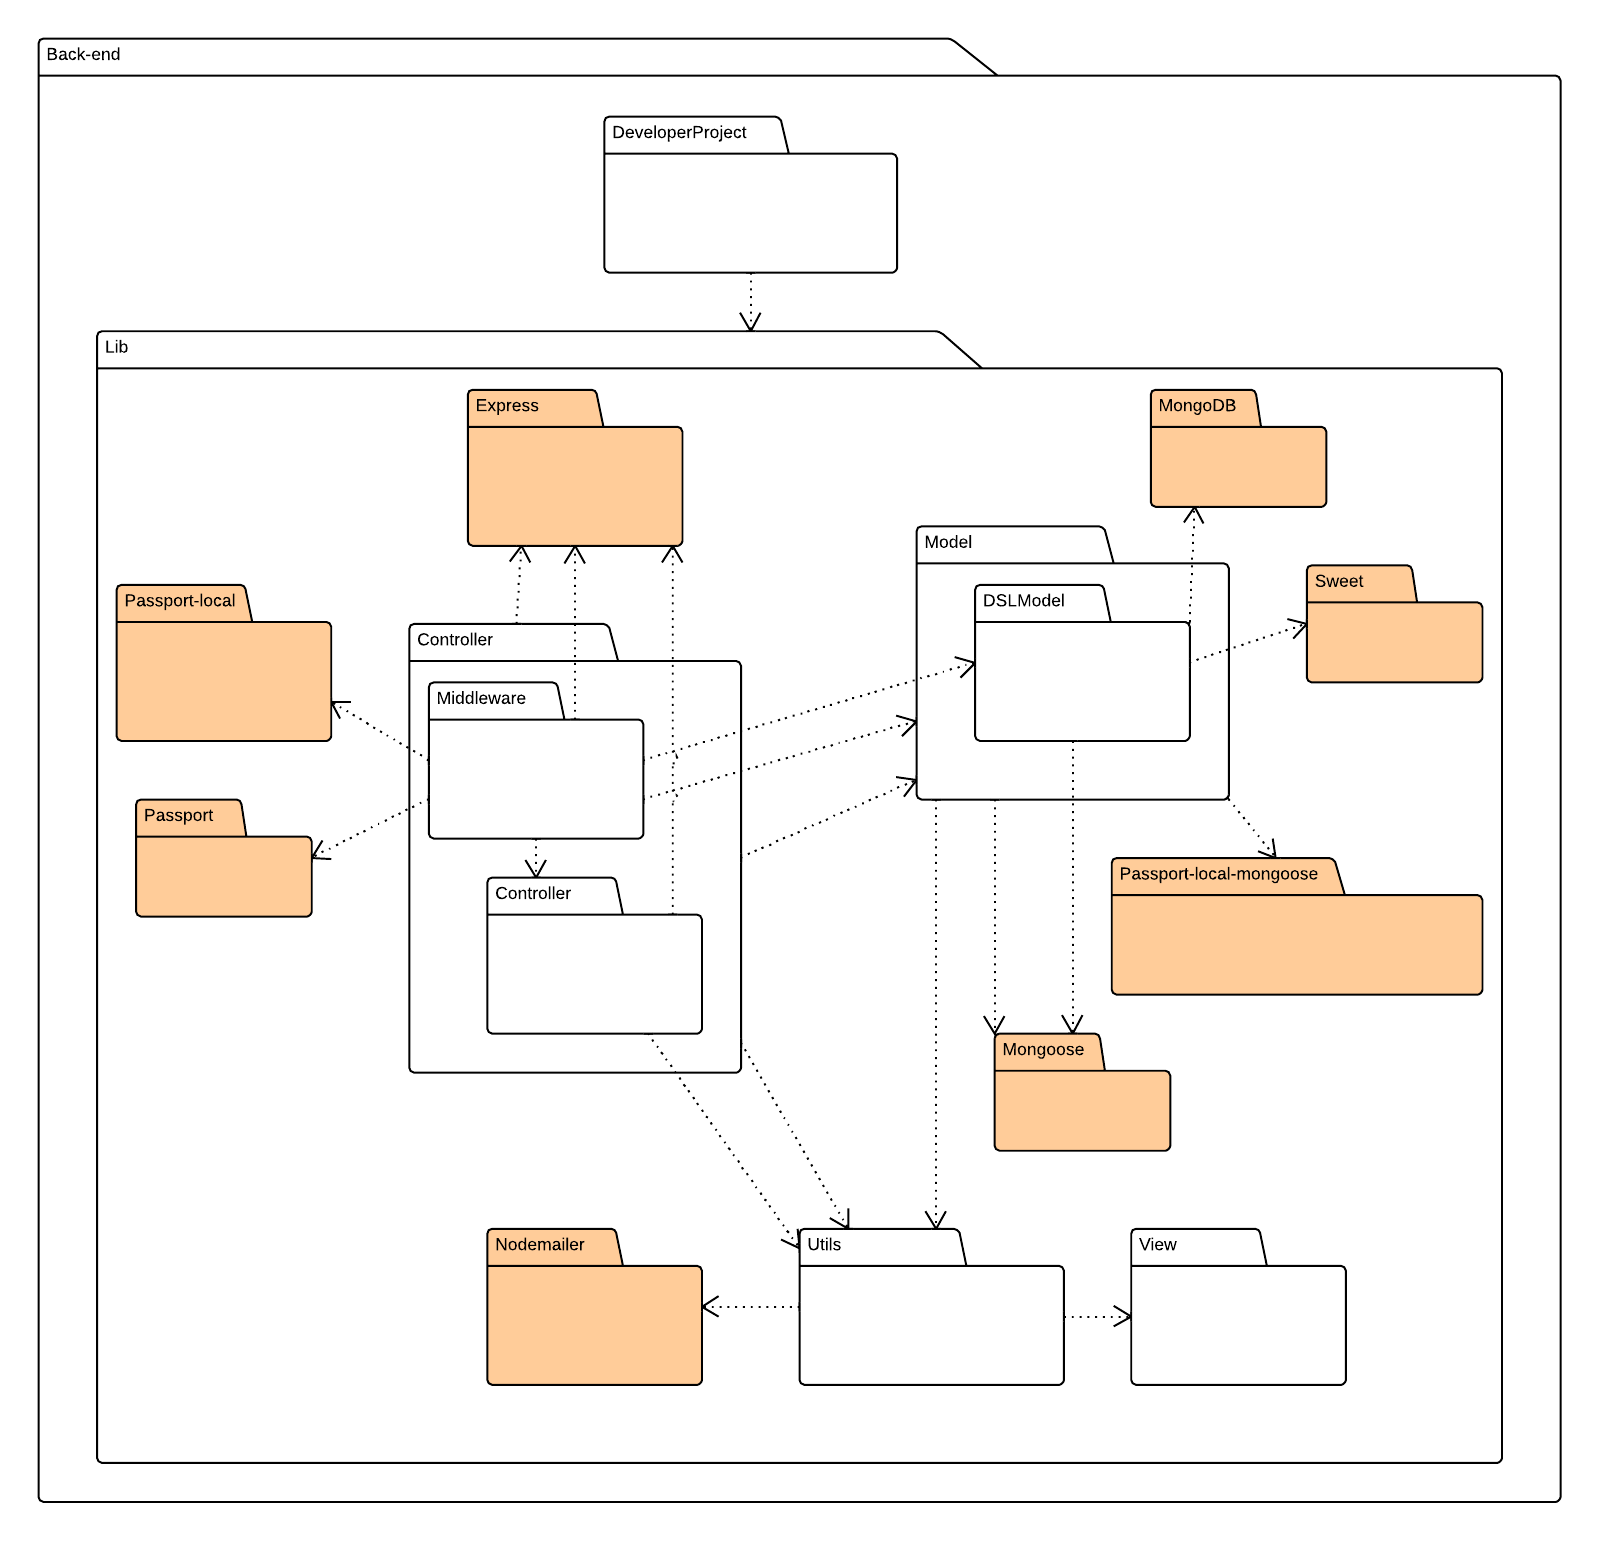
\includegraphics[width=\textwidth]{uml/package/Back-end.png}  
				\caption{Diagramma dei packages Back-end}
			\end{center}  
		\end{figure} 
		
		\begin{figure}[H] 
			\begin{center} 
				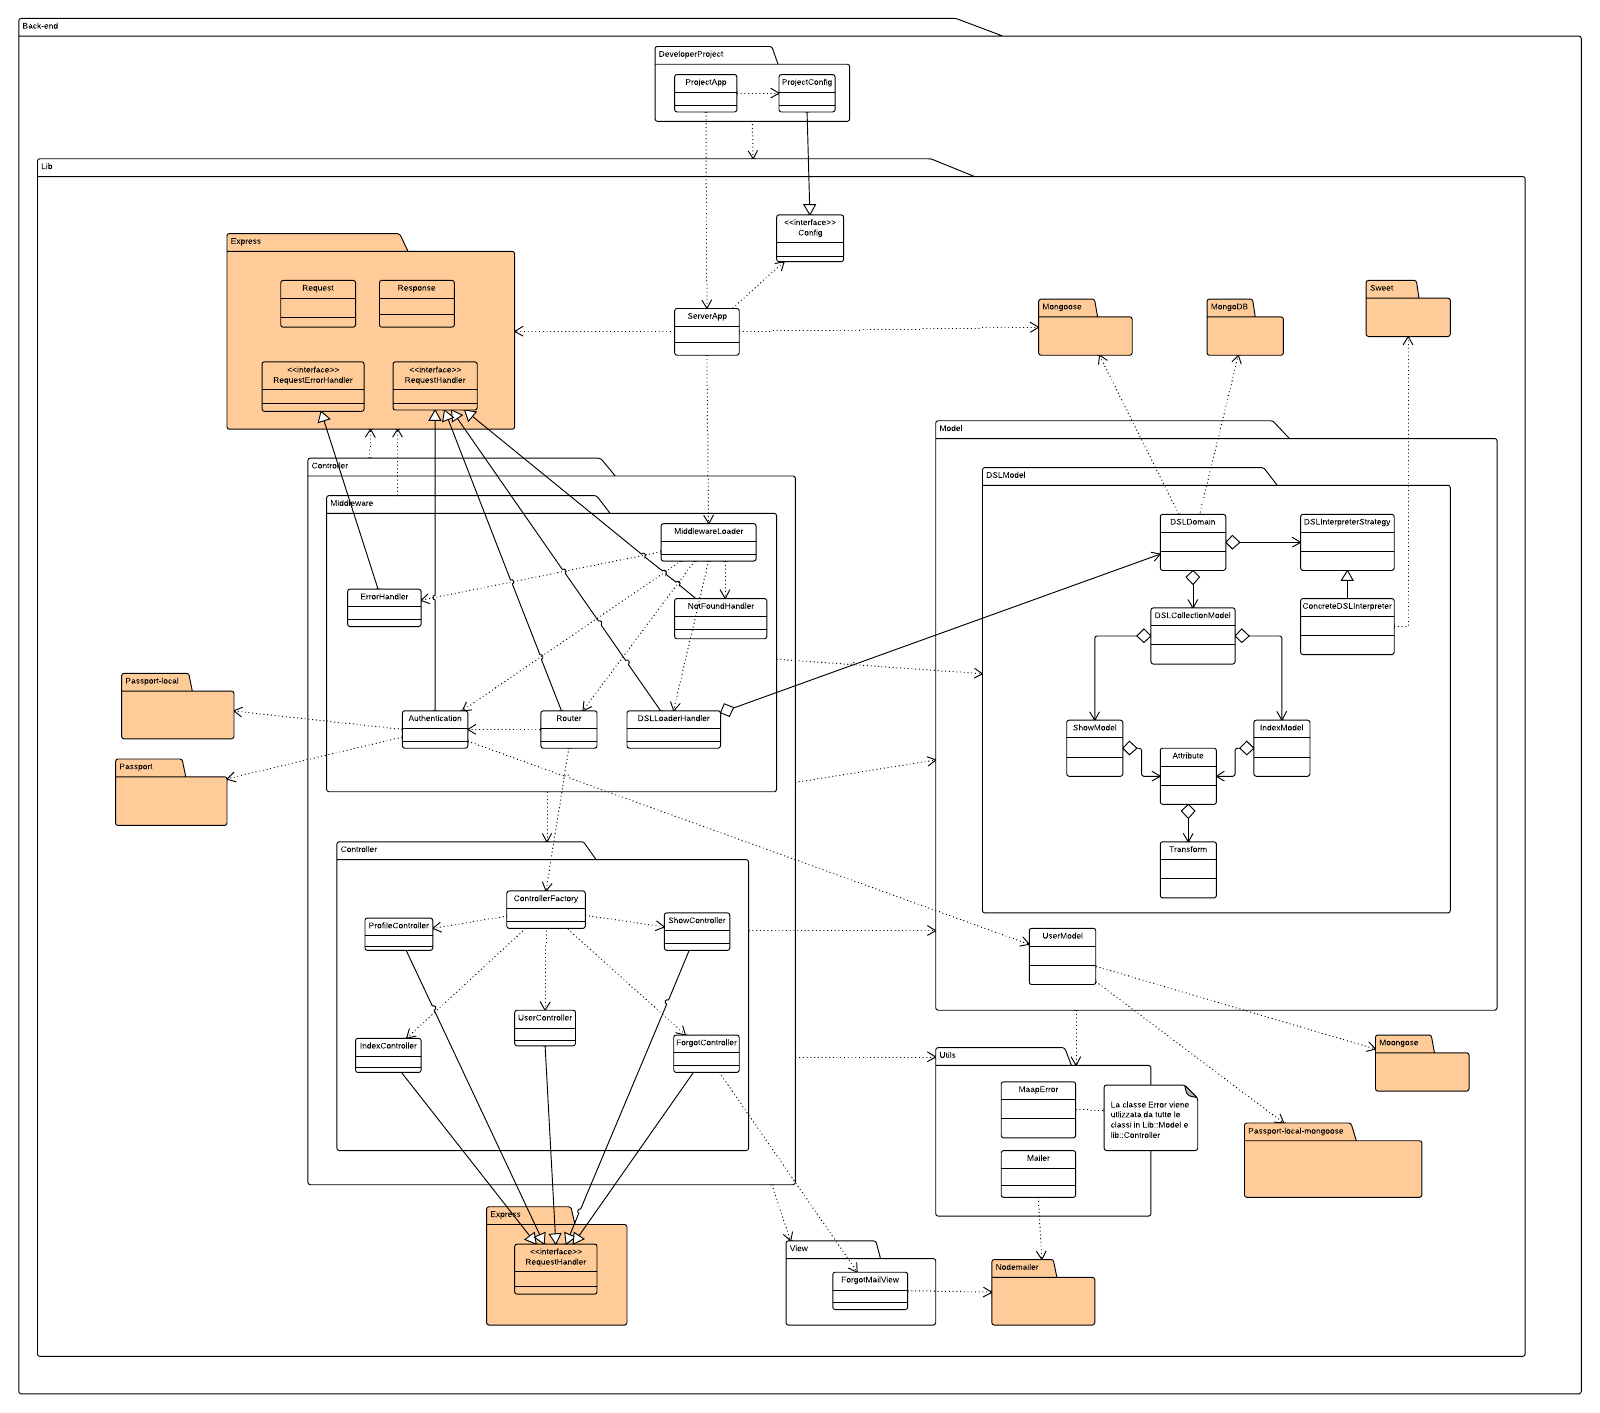
\includegraphics[width=\textwidth]{uml/classi/Back-end.png}  
				\caption{Diagramma delle classi Back-end}
			\end{center}  
		\end{figure} 
		
	\subparagraph{Descrizione} 
		\begin{itemize}
		\item[] \glossario{Package} che racchiude tutta la componente di \glossario{Back-end}. Comprende la libreria dell'applicazione \textit{MaaP} e il package del progetto sviluppato dal developer che andrà ad utilizzare tale libreria.
		\end{itemize} 
		\subparagraph{Package contenuti} 
		\begin{itemize}
				\item DeveloperProject
				\item Lib
		\end{itemize}
	\subsubsection{Back-end::DeveloperProject}
	\paragraph{Informazioni sul package} 
		\begin{figure}[H] 
			\begin{center} 
				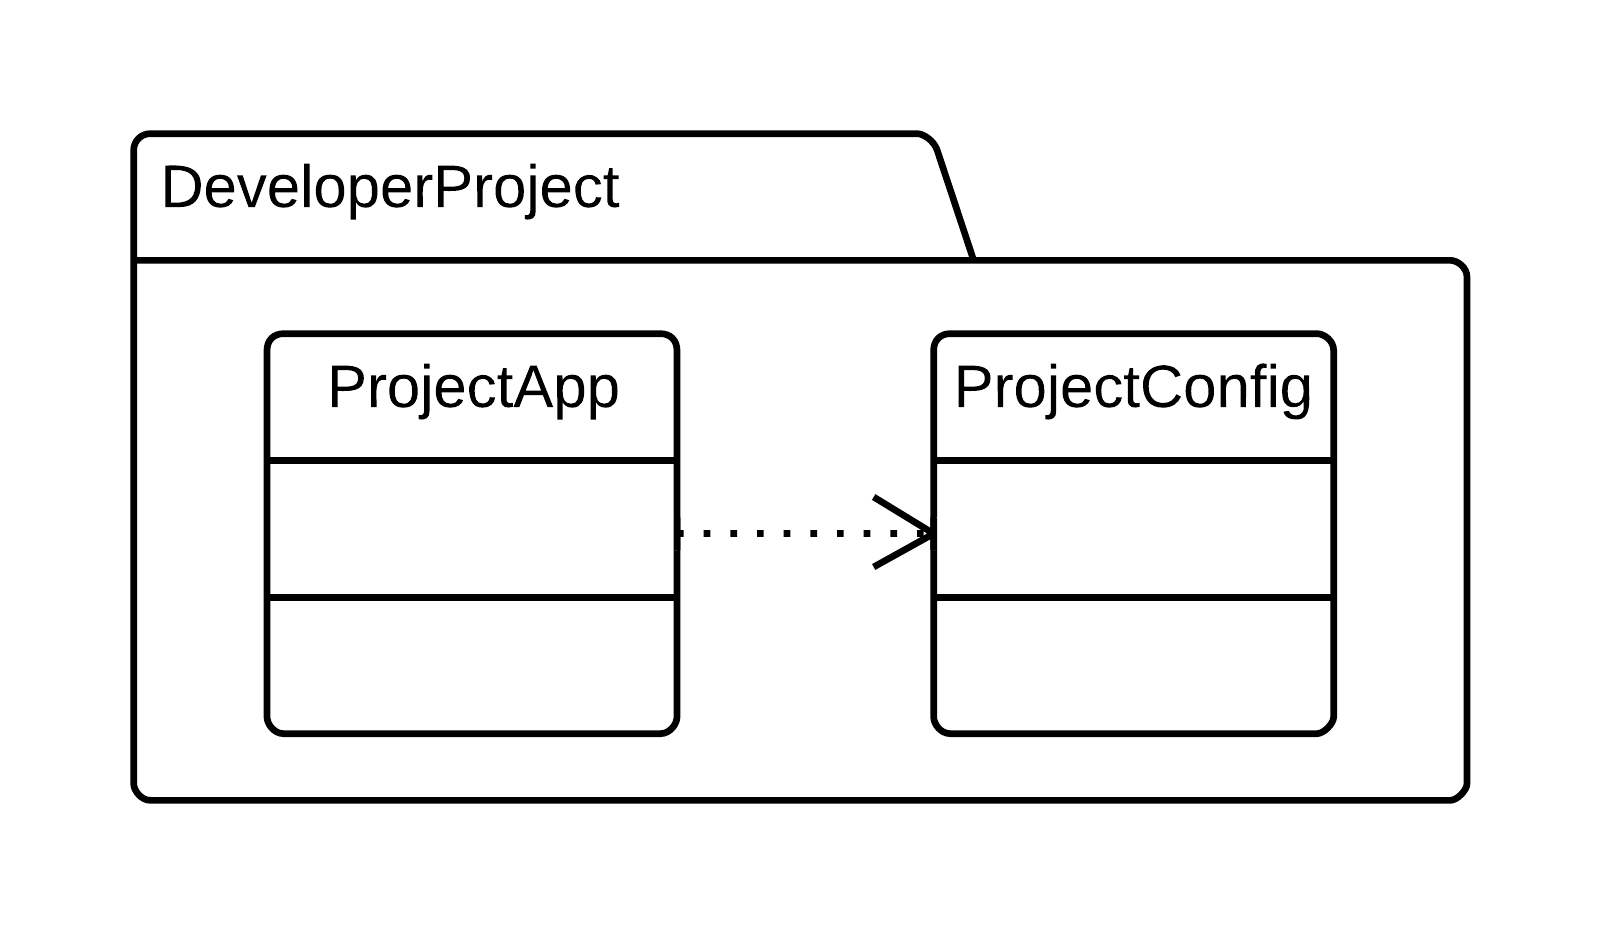
\includegraphics[scale=0.18]{uml/package/Back-end::DeveloperProject.png}  
				\caption{Componente DeveloperProject}
			\end{center}  
		\end{figure} 
	\subparagraph{Descrizione} 
		\begin{itemize}
		\item[] Questo \glossario{Package} ha il compito di fornire la configurazione e avviare il web server di \glossario{MaaP}. Consiste negli oggetti che dovranno essere predisposti dal developer che vorrà installare il framework \glossario{MaaP}. L'installazione dell framework \glossario{MaaP} fornisce uno \glossario{scaffold} dei file e delle classi necessarie per il funzionamento dell'applicazione. Sarà compito del developer modificare tali file inserendo i dati corretti.
		\end{itemize} 
	\subparagraph{Interazioni con altri componenti} 
		\begin{itemize} 
				\item Back-end::Lib  
		\end{itemize} 
		\paragraph{Classi}
			\subparagraph{ProjectConfig}
				
				\textbf{\\ \\ Descrizione} 
					\begin{itemize}
						\item[] Questa classe rappresenta la configurazione di un'applicazione.
					\end{itemize}      
				\textbf{Utilizzo}  
					\begin{itemize}
						\item[] Viene passato come parametro al costruttore della classe ServerApp per configurare l'applicazione.
					\end{itemize}
					\textbf{Classi Ereditate}
					\begin{itemize}
								\item{Back-end::Lib::Config}
					\end{itemize}
			\subparagraph{ProjectApp}
				
				\textbf{\\ \\ Descrizione} 
					\begin{itemize}
						\item[] Classe modificabile dall'utente-developer che si occupa di configurare e avviare il server dell'applicazione.
					\end{itemize}      
				\textbf{Utilizzo}  
					\begin{itemize}
						\item[] Internamente avvia il server utilizzando la classe ServerApp, a cui passa i parametri di configurazione del progetto definiti con un oggetto della classe ProjectConfig.
					\end{itemize}
					\textbf{Relazioni con altre classi}
					\begin{itemize}
							\item{Back-end::DeveloperProject::Config::ProjectConfig}
							\item{Back-end::Lib::ServerApp}
					\end{itemize}
	\subsubsection{Back-end::Lib}
	\paragraph{Informazioni sul package} 
		\begin{figure}[H] 
			\begin{center} 
				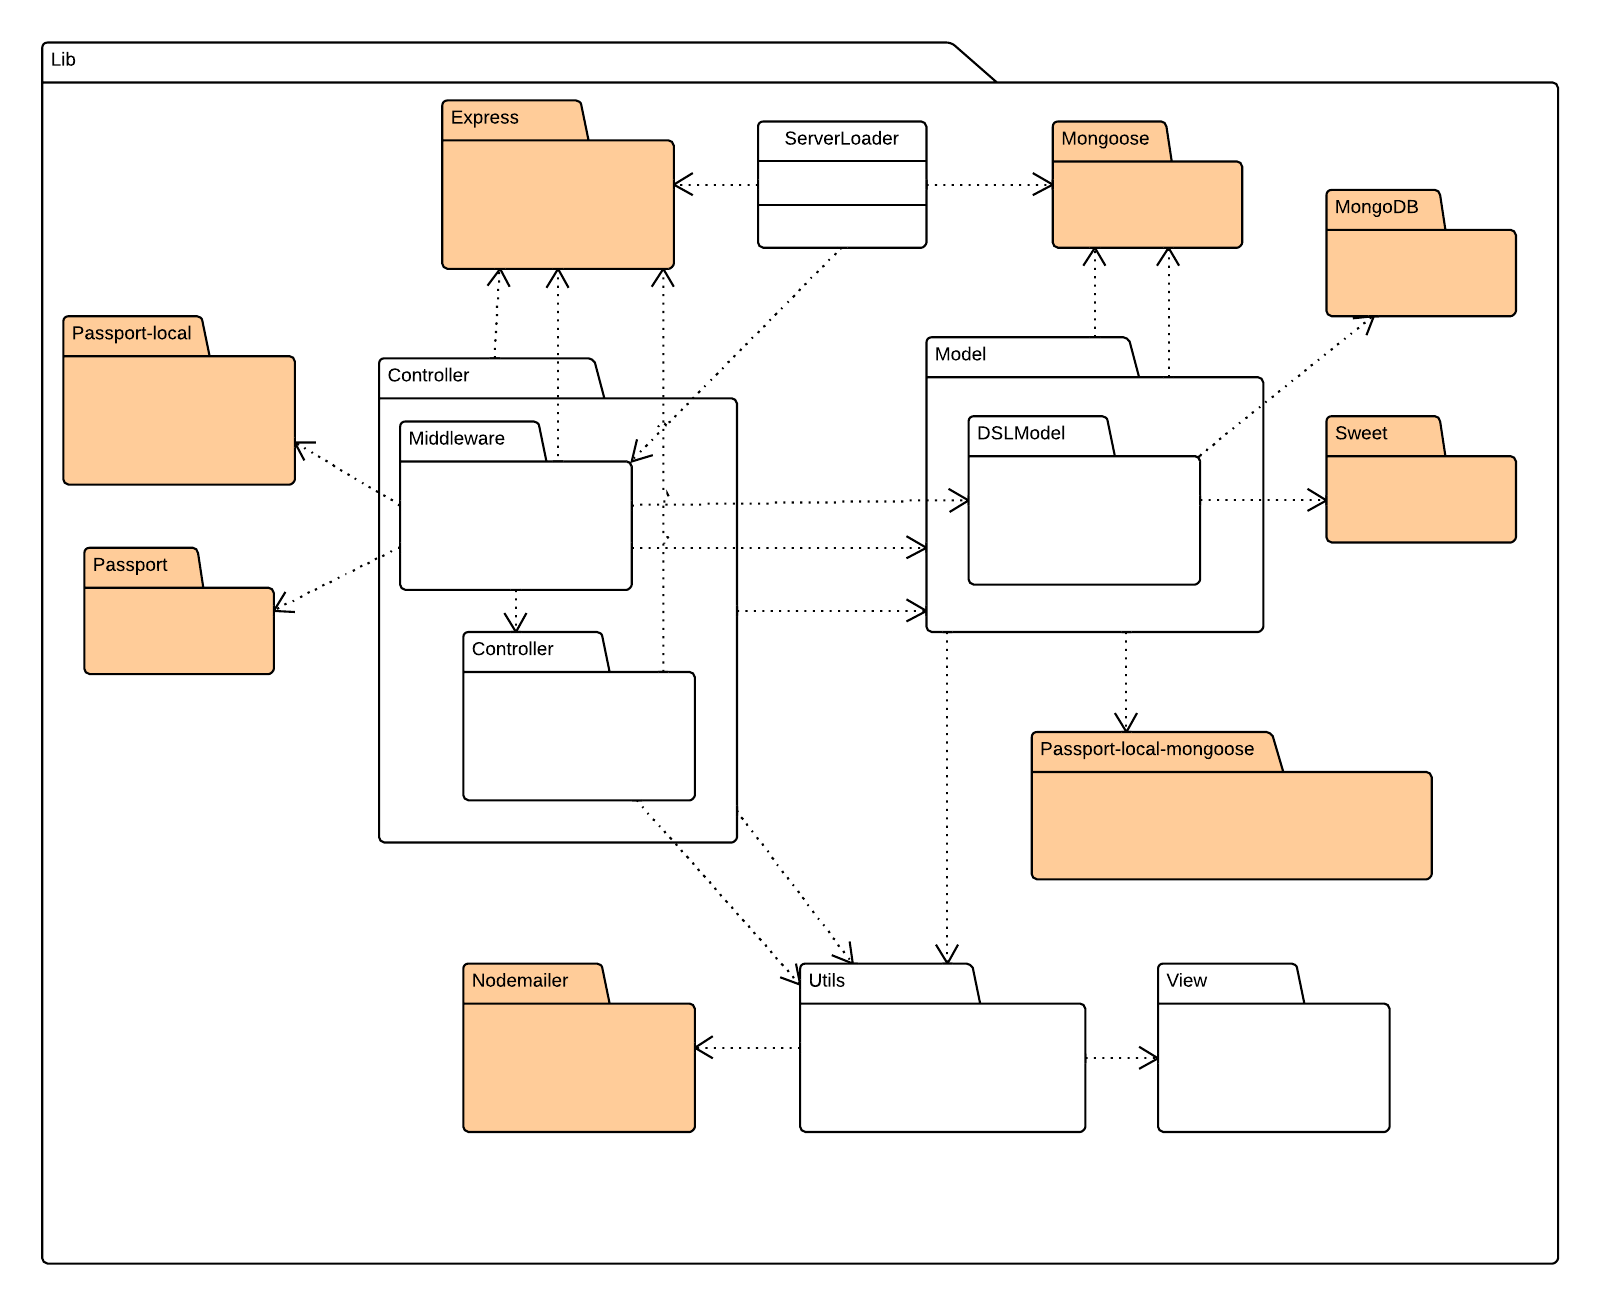
\includegraphics[scale=0.24]{uml/package/Back-end::Lib.png}  
				\caption{Componente Lib}
			\end{center}  
		\end{figure} 
	\subparagraph{Descrizione} 
		\begin{itemize}
		\item[] \glossario{Package} che costituisce la libreria principale dell’applicazione \glossario{MaaP}, che verrà fornita ai
developer per installare e utilizzare l’applicazione. Comprende gli script per l’installazione,
non rappresentati nei diagrammi in quanto non sono modellati come oggetti.

		\end{itemize} 
		\subparagraph{Package contenuti} 
		\begin{itemize}
				\item Controller
				\item Model
				\item View
				\item Utils
		\end{itemize}
		\paragraph{Classi}
			\subparagraph{Config}
				
				\textbf{\\ \\ Descrizione} 
					\begin{itemize}
						\item[] Classe che rappresenta l'interfaccia della classe di configurazione dell'applicazione.
					\end{itemize}      
				\textbf{Utilizzo}  
					\begin{itemize}
						\item[] Viene utilizzata per descrivere tutti i parametri dell'applicazione. Quando viene creata una ServerApp le viene passato un oggetto di questo tipo ed essa avvierà l'applicazione a partire da questa configurazione.
					\end{itemize}
					\textbf{Estensioni}
					\begin{itemize}
							\item{Back-end::DeveloperProject::Config::ProjectConfig}
					\end{itemize}
			\subparagraph{ServerApp}
				
				\textbf{\\ \\ Descrizione} 
					\begin{itemize}
						\item[] Classe che si occupa di avviare il server e di invocare il \glossario{middleware}. È il componente client del \glossario{Design Pattern} \glossario{Chain of responsibility}. Utilizza i pacchetti Mongoose ed Express.
					\end{itemize}      
				\textbf{Utilizzo}  
					\begin{itemize}
						\item[] Viene utilizzato per avviare l'applicazione. Internamente inizializza la catena gestione delle chiamate utilizzando la classe \texttt{Back-end::Lib::Middleware::MiddlewareLoader}.
					\end{itemize}
					\textbf{Relazioni con altre classi}
					\begin{itemize}
							\item{Back-end::Lib::Controller::Middleware::MiddlewareLoader}
							\item{Back-end::Lib::Config}
					\end{itemize}
	\subsubsection{Back-end::Lib::View}
	\paragraph{Informazioni sul package} 
		\begin{figure}[H] 
			\begin{center} 
				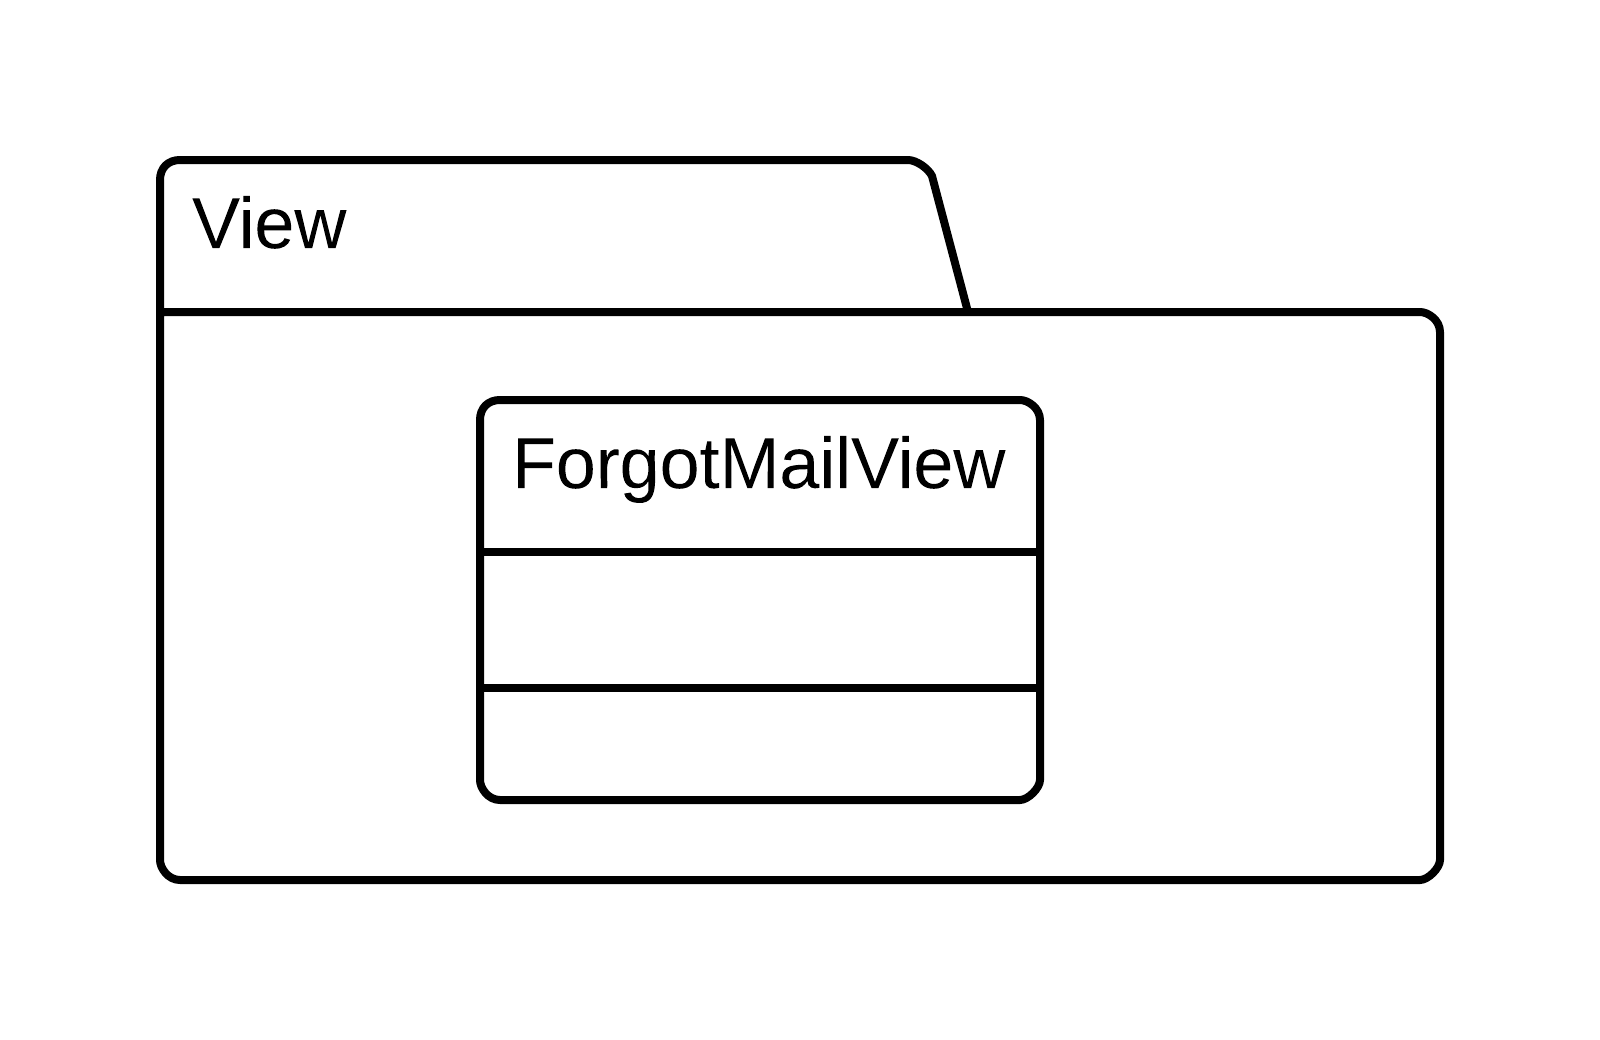
\includegraphics[scale=0.15]{uml/package/Back-end::Lib::View.png}  
				\caption{Componente View}
			\end{center}  
		\end{figure} 
	\subparagraph{Descrizione} 
		\begin{itemize}
		\item[] \glossario{Package} contenente le classi che costituiscono i template, utilizzati ad esempio per le email di recupero-
password.

		\end{itemize} 
		\paragraph{Classi}
			\subparagraph{ForgotMailView}
				
				\textbf{\\ \\ Descrizione} 
					\begin{itemize}
						\item[] Classe che fornisce una rappresentazione della mail.
					\end{itemize}      
				\textbf{Utilizzo}  
					\begin{itemize}
						\item[] Viene utilizzata come template di email da inviare nel caso in cui l'utente richieda il recupero password.
					\end{itemize}
	\subsubsection{Back-end::Lib::Controller}
	\paragraph{Informazioni sul package} 
		\begin{figure}[H] 
			\begin{center} 
				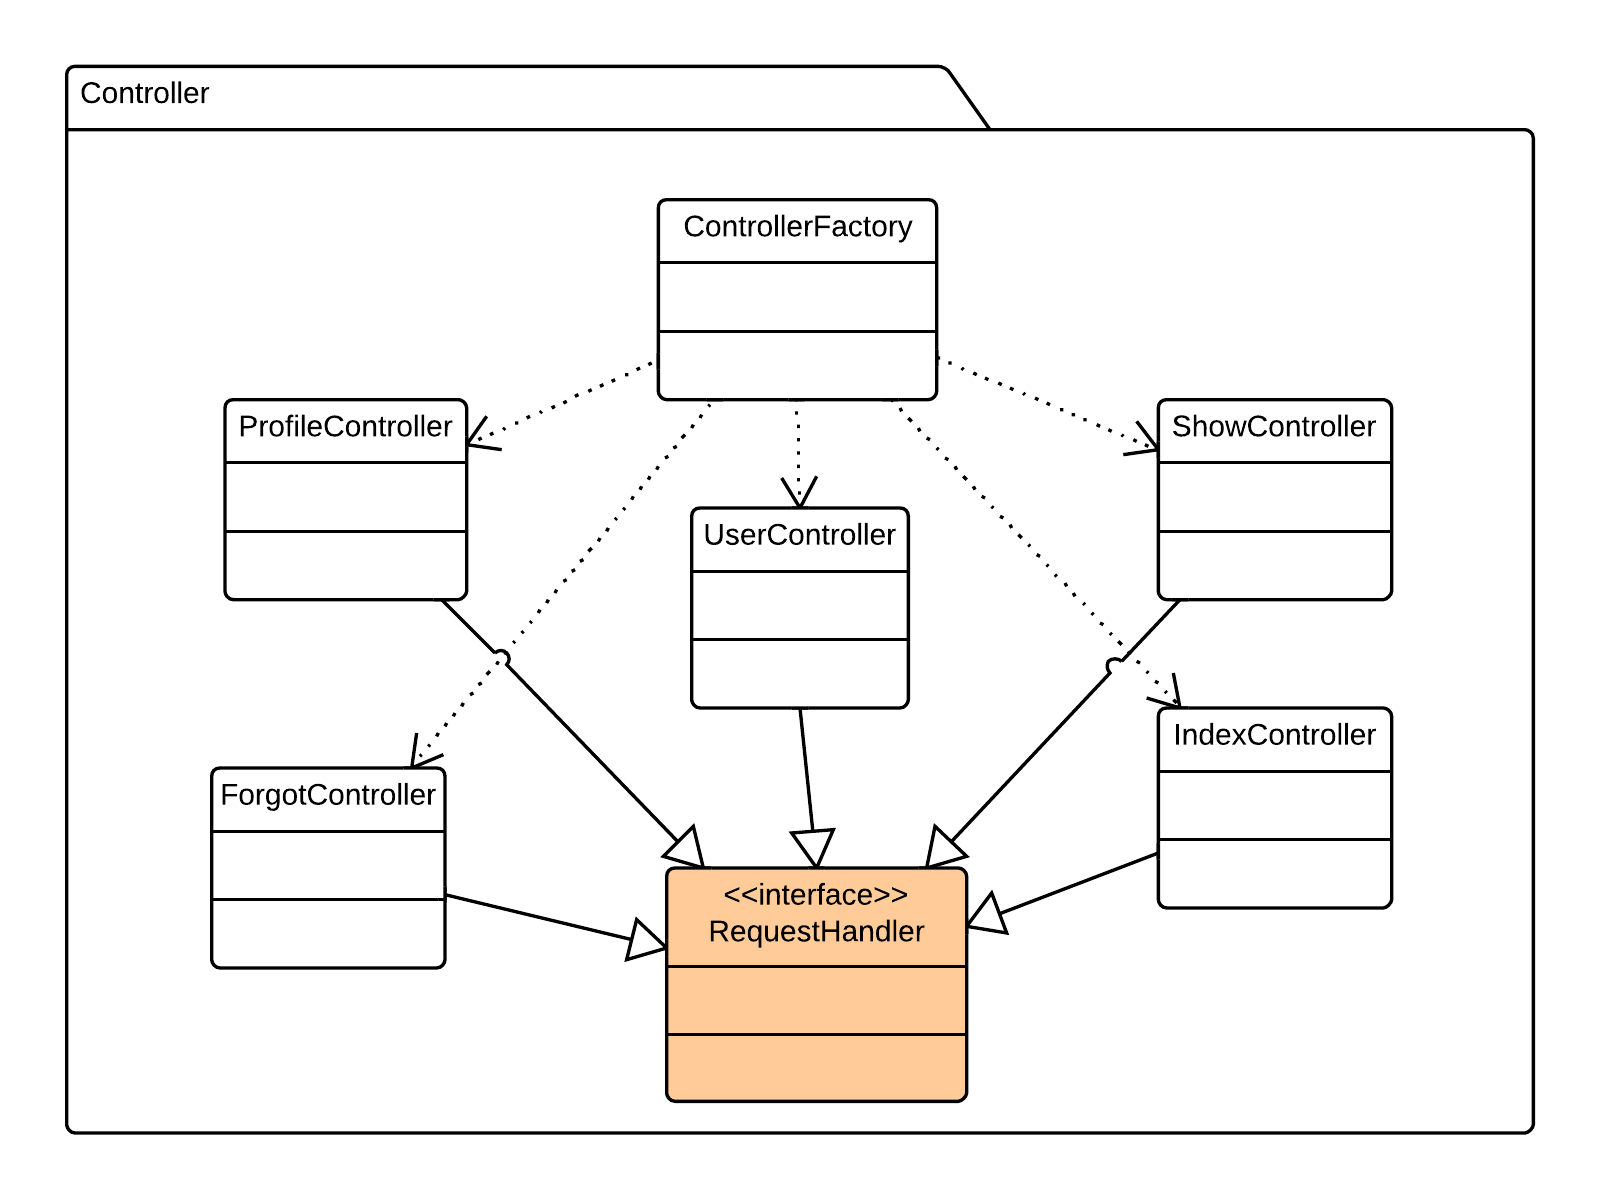
\includegraphics[scale=0.15]{uml/package/Back-end::Lib::Controller.png}  
				\caption{Componente Controller}
			\end{center}  
		\end{figure} 
	\subparagraph{Descrizione} 
		\begin{itemize}
		\item[] \glossario{Package} contenente le componenti che gestiscono la logica con cui vengono elaborate le richieste inviate all’applicazione.
		\end{itemize} 
		\subparagraph{Package contenuti} 
		\begin{itemize}
				\item Controller
				\item Middleware
		\end{itemize}
	\subsubsection{Back-end::Lib::Controller::Middleware}
	\paragraph{Informazioni sul package} 
		\begin{figure}[H] 
			\begin{center} 
				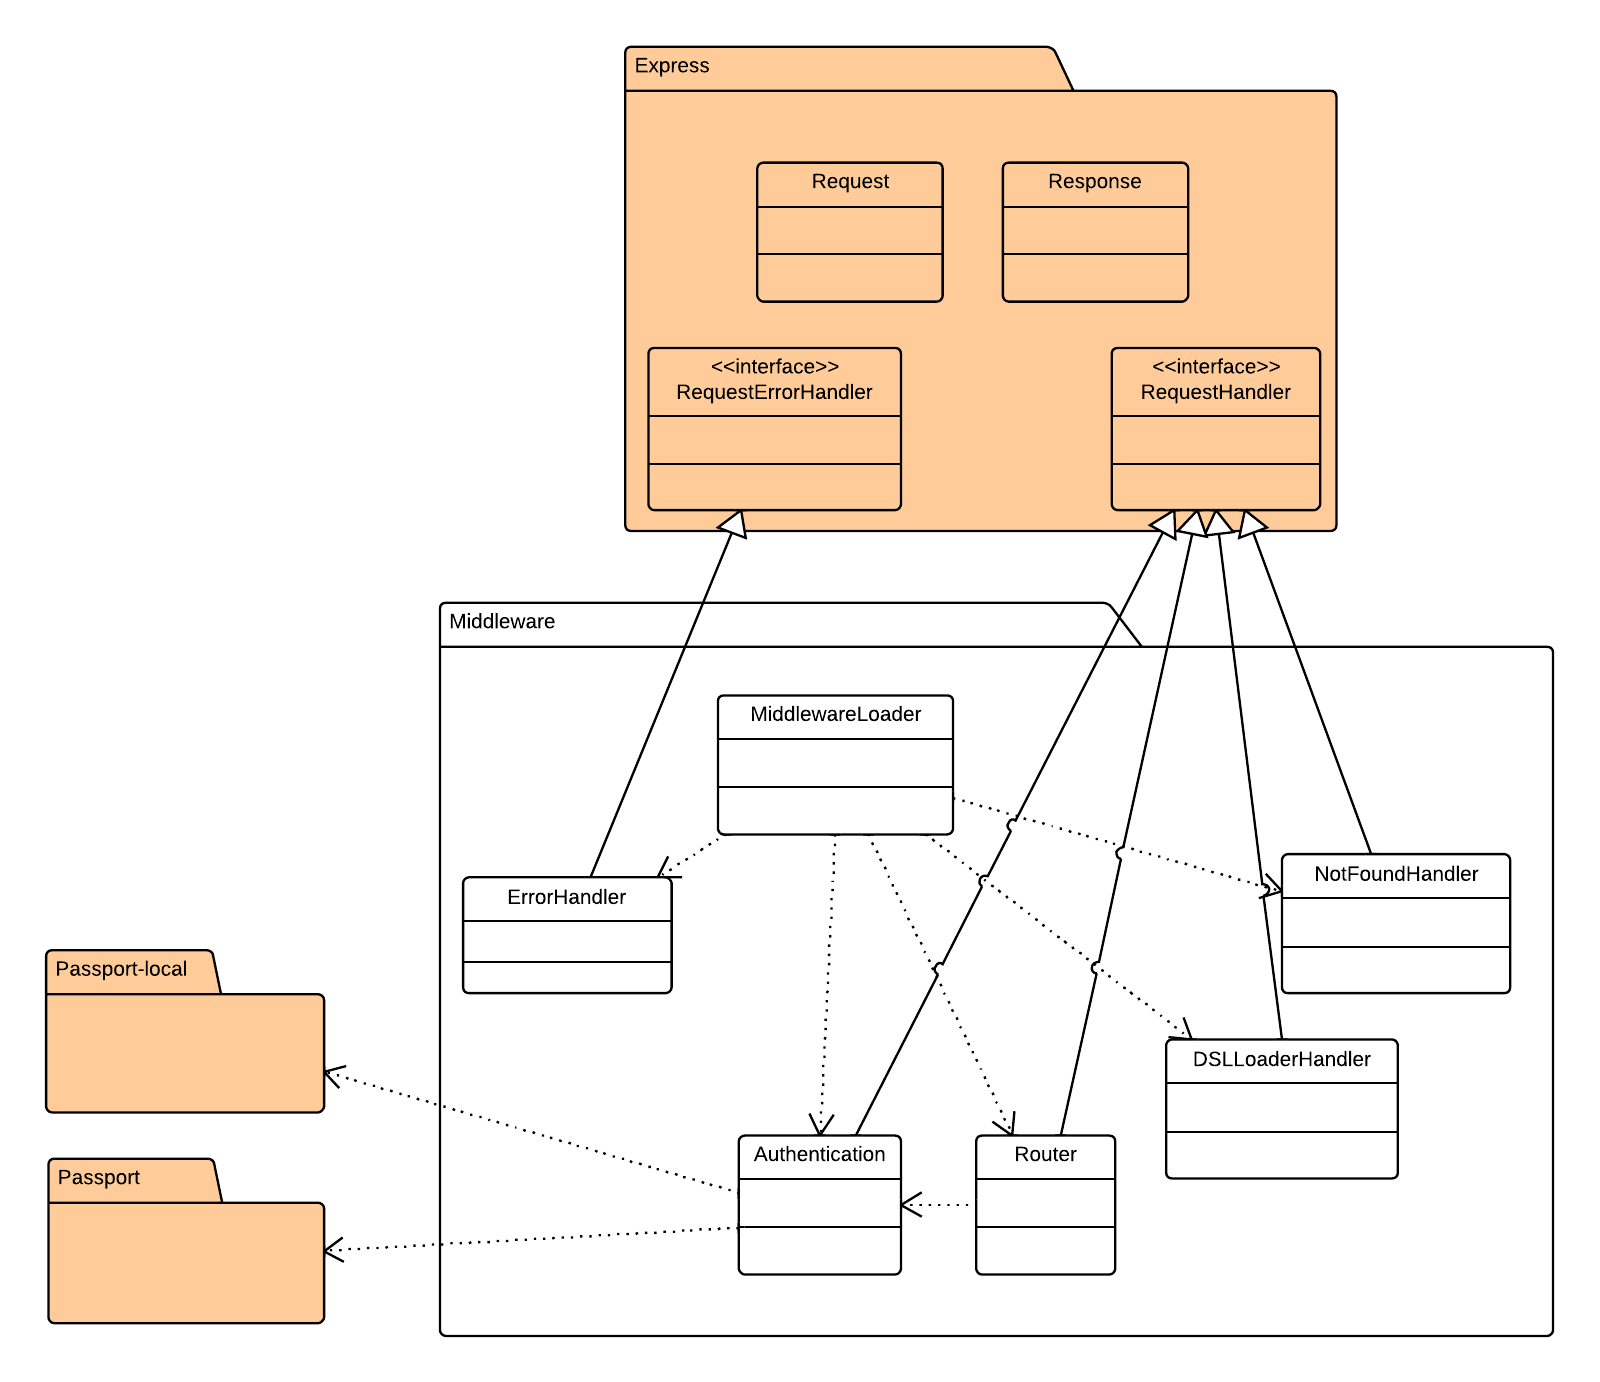
\includegraphics[width=\textwidth]{uml/package/Back-end::Lib::Controller::Middleware.png}  
				\caption{Componente Middleware}
			\end{center}  
		\end{figure} 
	\subparagraph{Descrizione} 
		\begin{itemize}
		\item[] \glossario{Package} contenente classi che costituiscono gli handler della catena di chiamate a cui viene
passata la responsabilità di gestire una richiesta, decorando quest’ultima con parametri e
metodi utilizzabili dai controller. Costituisce una parte controller nell’architettura \glossario{MVC}
del \glossario{Back-end} .

		\end{itemize} 
	\subparagraph{Interazioni con altri componenti} 
		\begin{itemize} 
				\item Back-end::Lib::Model
				\item Back-end::Lib::Controller::Controller
				\item Back-end::Lib::Model::DSLModel  
		\end{itemize} 
		\paragraph{Classi}
			\subparagraph{Authentication}
				
				\textbf{\\ \\ Descrizione} 
					\begin{itemize}
						\item[] Classe che si occupa dell'autenticazione di un'utente. È uno dei componenti subsystem class del \glossario{Design Pattern} \glossario{Facade} e handler del \glossario{Design Pattern} \glossario{Chain of responsibility}.
					\end{itemize}      
				\textbf{Utilizzo}  
					\begin{itemize}
						\item[] Viene utilizzata per verificare i dati inseriti dall'utente nella pagina di login e controllare l'effettiva corrispondenza delle credenziali nel \glossario{database}.
					\end{itemize}
					\textbf{Relazioni con altre classi}
					\begin{itemize}
							\item{Back-end::Lib::Model::UserModel}
					\end{itemize}
			\subparagraph{MiddlewareLoader}
				
				\textbf{\\ \\ Descrizione} 
					\begin{itemize}
						\item[] Classe che definisce un'interfaccia comune per tutte le richieste dell'applicazione. È la componente facade del \glossario{Design Pattern} \glossario{Facade} e handler del \glossario{Design Pattern} \glossario{Chain of responsibility}.
					\end{itemize}      
				\textbf{Utilizzo}  
					\begin{itemize}
						\item[] Viene utilizzato per istanziare in modo "nascosto" all'applicazione tutti i \glossario{middleware} presenti nel componente \texttt{Back-end::Lib::Middleware}.
					\end{itemize}
					\textbf{Relazioni con altre classi}
					\begin{itemize}
							\item{Back-end::Lib::Controller::Middleware::Authentication}
							\item{Back-end::Lib::Controller::Middleware::DSLLoaderHandler}
							\item{Back-end::Lib::Controller::Middleware::NotFoundHandler}
							\item{Back-end::Lib::Controller::Middleware::ErrorHandler}
							\item{Back-end::Lib::Controller::Middleware::Router}
					\end{itemize}
			\subparagraph{DSLLoaderHandler}
				
				\textbf{\\ \\ Descrizione} 
					\begin{itemize}
						\item[] Classe che si occupa di caricare i \glossario{DSL} presenti nel sistema. È uno dei componenti subsystem class del \glossario{Design Pattern} \glossario{Facade} e handler del \glossario{Design Pattern} \glossario{Chain of responsibility}.
					\end{itemize}      
				\textbf{Utilizzo}  
					\begin{itemize}
						\item[] Viene utilizzata per caricare i \glossario{DSL} delle \glossario{Collection} all'interno del \glossario{database}.
					\end{itemize}
					\textbf{Relazioni con altre classi}
					\begin{itemize}
							\item{Back-end::Lib::Model::DSLModel::DSLDomain}
					\end{itemize}
			\subparagraph{NotFoundHandler}
				
				\textbf{\\ \\ Descrizione} 
					\begin{itemize}
						\item[] Classe che si occupa la gestione dell'errore di pagina non trovata. È uno dei componenti subsystem class del \glossario{Design Pattern} \glossario{Facade} e handler del \glossario{Design Pattern} \glossario{Chain of responsibility}.
					\end{itemize}      
				\textbf{Utilizzo}  
					\begin{itemize}
						\item[] Viene utilizzata per generare una pagina 404 di errore nel caso in cui l'\glossario{URI} passato non corrisponda ad una risorsa presente nell'applicazione.
					\end{itemize}
			\subparagraph{ErrorHandler}
				
				\textbf{\\ \\ Descrizione} 
					\begin{itemize}
						\item[] Questa classe gestisce gli errori generati nei precedenti middleware o controller. Invia al client una risposta con stato HTTP 500 (server error) con una descrizione dell'errore nel formato JSON.
È uno dei componenti subsystem class del \glossario{Design Pattern} \glossario{Facade} e handler del \glossario{Design Pattern} \glossario{Chain of responsibility}.
					\end{itemize}      
				\textbf{Utilizzo}  
					\begin{itemize}
						\item[] Questo middleware viene utilizzato per ultimo nella catena di gestione delle richieste di Express, in modo da gestire tutti gli errori generati precedentemente.
					\end{itemize}
			\subparagraph{Router}
				
				\textbf{\\ \\ Descrizione} 
					\begin{itemize}
						\item[] Classe che si occupa della richiesta di risorse. È uno dei componenti subsystem class del \glossario{Design Pattern} \glossario{Facade} e handler del \glossario{Design Pattern} \glossario{Chain of responsibility}. Ha una relazione con la classe Authentication, poiché fa uso di alcuni metodi per controllare l'autenticazione.
					\end{itemize}      
				\textbf{Utilizzo}  
					\begin{itemize}
						\item[] Si occupa di smistare la richiesta in base all'\glossario{URI} ricevuto e ad invocare l'opportuno metodo di creazione sulla classe \texttt{Back-end::Lib::Controller::ControllerFactory}.
					\end{itemize}
					\textbf{Relazioni con altre classi}
					\begin{itemize}
							\item{Back-end::Lib::Controller::Controller::ControllerFactory}
							\item{Back-end::Lib::Utils::MaapError}
					\end{itemize}
	\subsubsection{Back-end::Lib::Controller::Controller}
	\paragraph{Informazioni sul package} 
		\begin{figure}[H] 
			\begin{center} 
				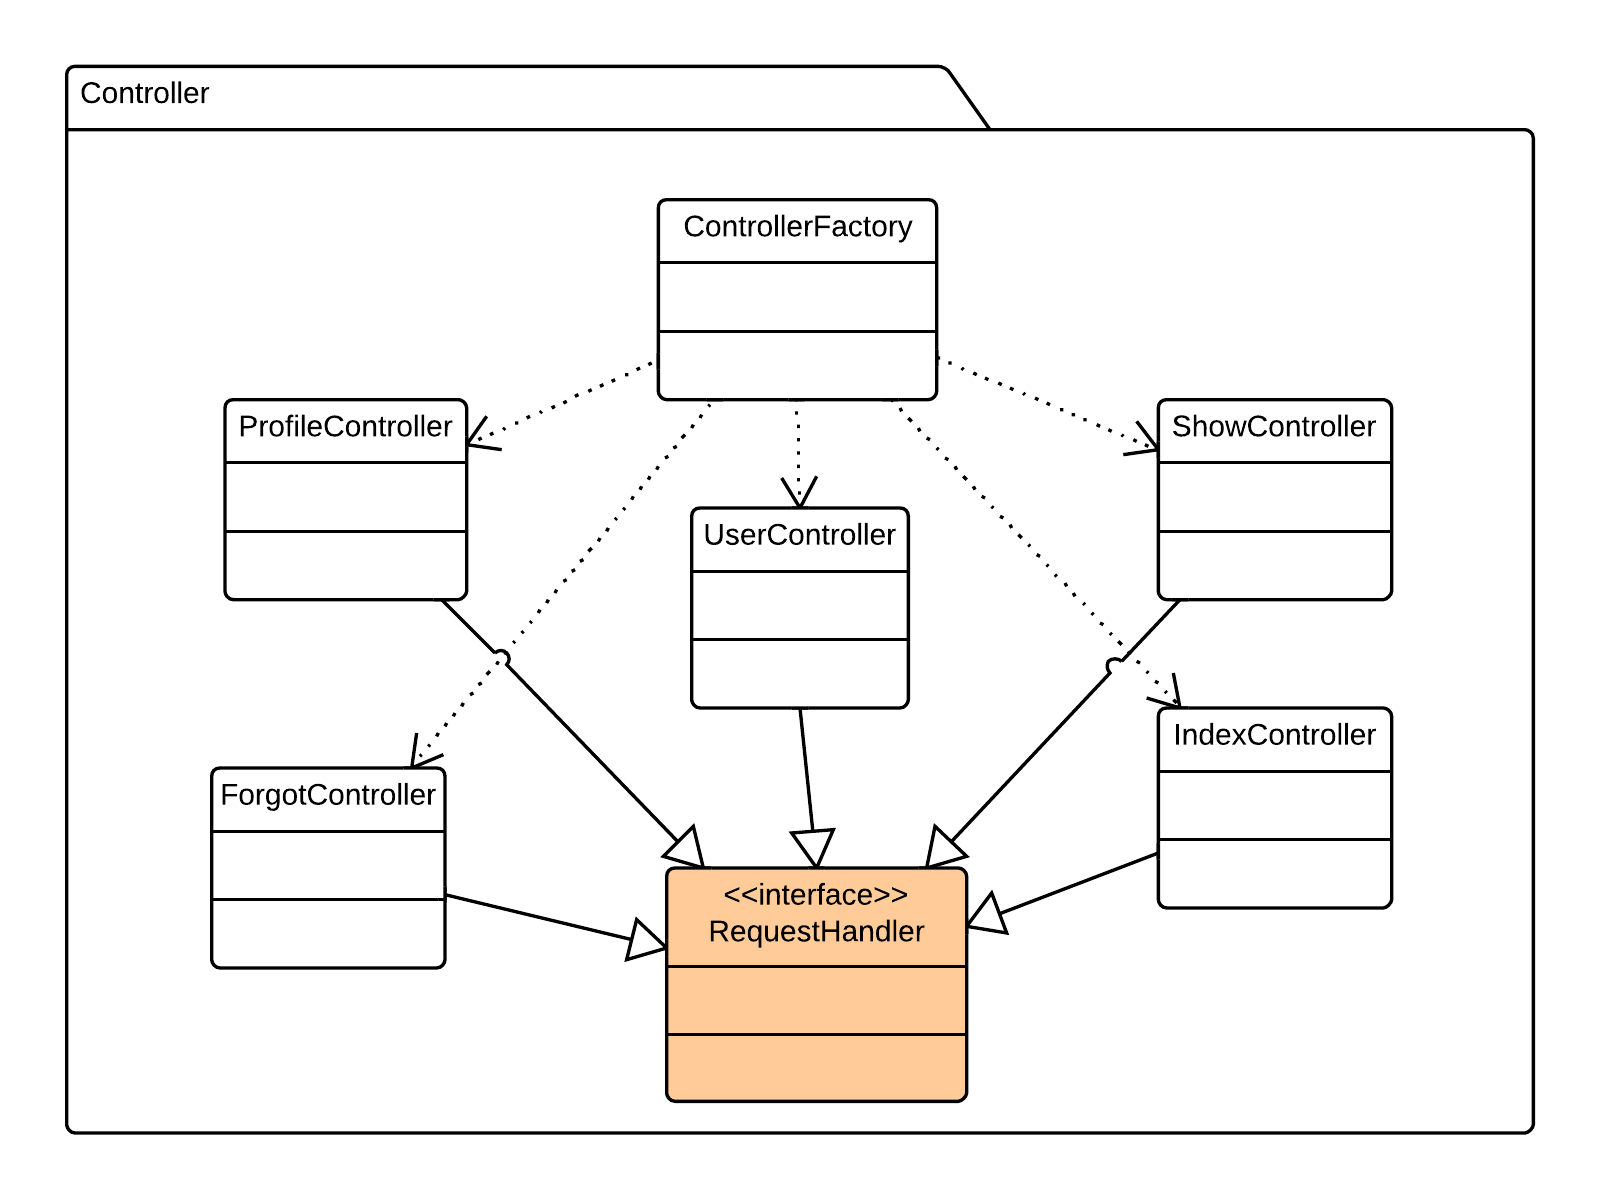
\includegraphics[scale=0.2]{uml/package/Back-end::Lib::Controller::Controller.png}  
				\caption{Componente Controller}
			\end{center}  
		\end{figure} 
	\subparagraph{Descrizione} 
		\begin{itemize}
		\item[] \glossario{Package} per il componente che realizza parte controller nell’architettura mvc nel back-
end. Contiene classi per le funzionalità di controllo e visualizzazione delle risorse, dove ogni
classe gestisce in modo esclusivo una sola di queste, in base all’ \glossario{URI} .

		\end{itemize} 
	\subparagraph{Interazioni con altri componenti} 
		\begin{itemize} 
				\item Back-end::Lib::View
				\item Back-end::Lib::Utils  
		\end{itemize} 
		\paragraph{Classi}
			\subparagraph{UserController}
				
				\textbf{\\ \\ Descrizione} 
					\begin{itemize}
						\item[] Classe che si occupa della varie operazioni che l'admin può compiere sugli utenti dell'applicazione. È uno dei componenti product del \glossario{Design Pattern} \glossario{Factory method}.
					\end{itemize}      
				\textbf{Utilizzo}  
					\begin{itemize}
						\item[] Viene utilizzata per visualizzare la \glossario{index-page} degli utenti, visualizzare le relative \glossario{show-page}, eliminare un utente e modificare il profilo. Mette a disposizione dei metodi per effettuare tutte queste operazioni.
					\end{itemize}
			\subparagraph{IndexController}
				
				\textbf{\\ \\ Descrizione} 
					\begin{itemize}
						\item[] Classe di gestione per la risorsa index 
È uno dei componenti product del \glossario{Design Pattern} \glossario{Factory method}.

					\end{itemize}      
				\textbf{Utilizzo}  
					\begin{itemize}
						\item[] Viene utilizzata per gestire la risorsa corrispondente all'index-page di un \glossario{Document}, offrendo metodi per restituirne gli attributi, effettuarne la modifica o la cancellazione e delega la visualizzazione dell'index-page alla classe \texttt{Back-end::Lib::DSLModel::DSLDomain}.

					\end{itemize}
			\subparagraph{ControllerFactory}
				
				\textbf{\\ \\ Descrizione} 
					\begin{itemize}
						\item[] Classe che si occupa di istanziare e restituire una classe \textit{Controller}. Rappresenta il componente creator del \glossario{Design Pattern} \glossario{Factory method}.
					\end{itemize}      
				\textbf{Utilizzo}  
					\begin{itemize}
						\item[] Viene costruita una sola volta dalla classe \textit{Back-end::Lib::Middleware::Router} e si occupa di creare e restituire l'oggetto \textit{Controller} richiesto.
					\end{itemize}
					\textbf{Relazioni con altre classi}
					\begin{itemize}
							\item{Back-end::Lib::Controller::Controller::UserController}
							\item{Back-end::Lib::Controller::Controller::IndexController}
							\item{Back-end::Lib::Controller::Controller::ShowController}
							\item{Back-end::Lib::Controller::Controller::ProfileController}
							\item{Back-end::Lib::Controller::Controller::ForgotController}
					\end{itemize}
			\subparagraph{ShowController}
				
				\textbf{\\ \\ Descrizione} 
					\begin{itemize}
						\item[] Classe che si occupa della gestione della risorsa show-page. È uno dei componenti \textit{product} del \glossario{Design Pattern} \glossario{Factory method}.
					\end{itemize}      
				\textbf{Utilizzo}  
					\begin{itemize}
						\item[] Viene utilizzata per gestire una richiesta della risorsa show-page, delegando alla classe \textit{Back-end::Lib::DSLModel::DSLDomain} il compito di eseguire la query e restituire i dati in formato JSON.
					\end{itemize}
			\subparagraph{ProfileController}
				
				\textbf{\\ \\ Descrizione} 
					\begin{itemize}
						\item[] Classe che rappresenta la gestione di un profilo utente, il login e il logout. È uno dei componenti product del \glossario{Design Pattern} \glossario{Factory method}.

					\end{itemize}      
				\textbf{Utilizzo}  
					\begin{itemize}
						\item[] Viene utilizzata per visualizzare il profilo dell'utente, tramite GET, e per editarlo tramite PUT. Viene anche utilizzata per gestire i dati di e le operazioni relativi all'autenticazione utente e al suo logout dall'applicazione, occupandosi della creazione della sessione utente e della sua distruzione tramite \glossario{cookies}.
					\end{itemize}
			\subparagraph{ForgotController}
				
				\textbf{\\ \\ Descrizione} 
					\begin{itemize}
						\item[] Classe che rappresenta il sistema di recupero e ripristino password. È uno dei componenti product del \glossario{Design Pattern} \glossario{Factory method}.
					\end{itemize}      
				\textbf{Utilizzo}  
					\begin{itemize}
						\item[] La classe fornisce dei metodi per effettuare una richiesta di reset password e, in un secondo momento, procedere al suo ripristino. La richiesta di reset avviene mandando un'email all'indirizzo dell'utente tramite la classe \texttt{Back-end::Lib::Middleware::Mailer}. All'interno di questo messaggio sarà presente un link che procederà ad effettuare il login dell'utente e a reindirizzarlo nella pagina di modifica profilo, dalla quale potrà modificare la password.
					\end{itemize}
					\textbf{Relazioni con altre classi}
					\begin{itemize}
							\item{Back-end::Lib::View::ForgotMailView}
					\end{itemize}
	\subsubsection{Back-end::Lib::Model}
	\paragraph{Informazioni sul package} 
		\begin{figure}[H] 
			\begin{center} 
				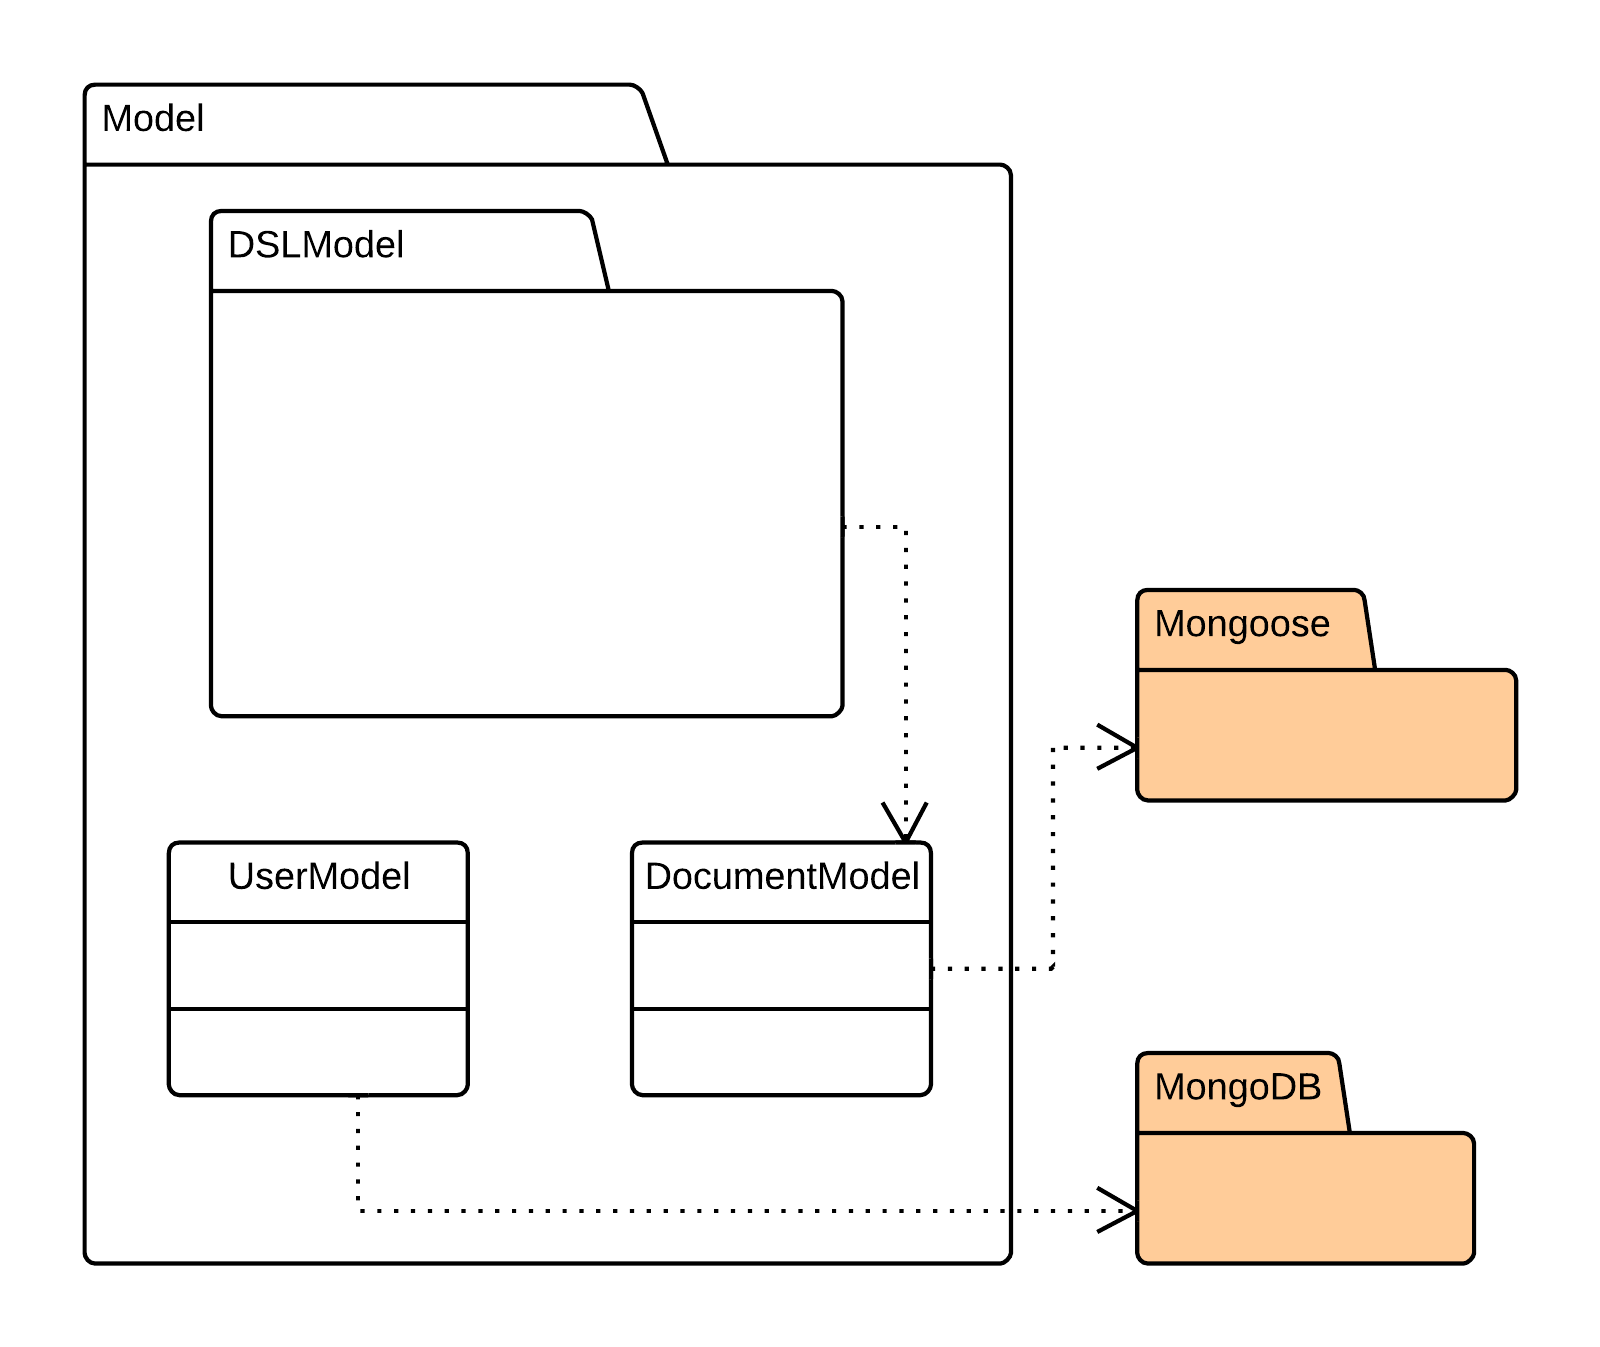
\includegraphics[scale=0.16]{uml/package/Back-end::Lib::Model.png}  
				\caption{Componente Model}
			\end{center}  
		\end{figure} 
	\subparagraph{Descrizione} 
		\begin{itemize}
		\item[] \glossario{Package} contenente le componenti che gestiscono i dati utilizzati dall’applicazione e l’interfacciamento con il
database
		\end{itemize} 
		\subparagraph{Package contenuti} 
		\begin{itemize}
				\item DSLModel
		\end{itemize}
		\paragraph{Classi}
			\subparagraph{UserModel}
				
				\textbf{\\ \\ Descrizione} 
					\begin{itemize}
						\item[] Classe che si occupa dei metodi per la gestione dei dati utente. 
					\end{itemize}      
				\textbf{Utilizzo}  
					\begin{itemize}
						\item[] Viene utilizzata per l'interfacciamento con la libreria \glossario{Mongoose} per la registrazione dello schema dei dati, e con la libreria passport-local-mongoose per il popolamento automatico dello schema con campi dati e metodi predefiniti.
Il costruttore del modello dello schema dei dati viene registrato nella \glossario{Factory} di \glossario{Mongoose} ed ogni istanza condividerà la stessa connessione al server.
					\end{itemize}
	\subsubsection{Back-end::Lib::Model::DSLModel}
	\paragraph{Informazioni sul package} 
		\begin{figure}[H] 
			\begin{center} 
				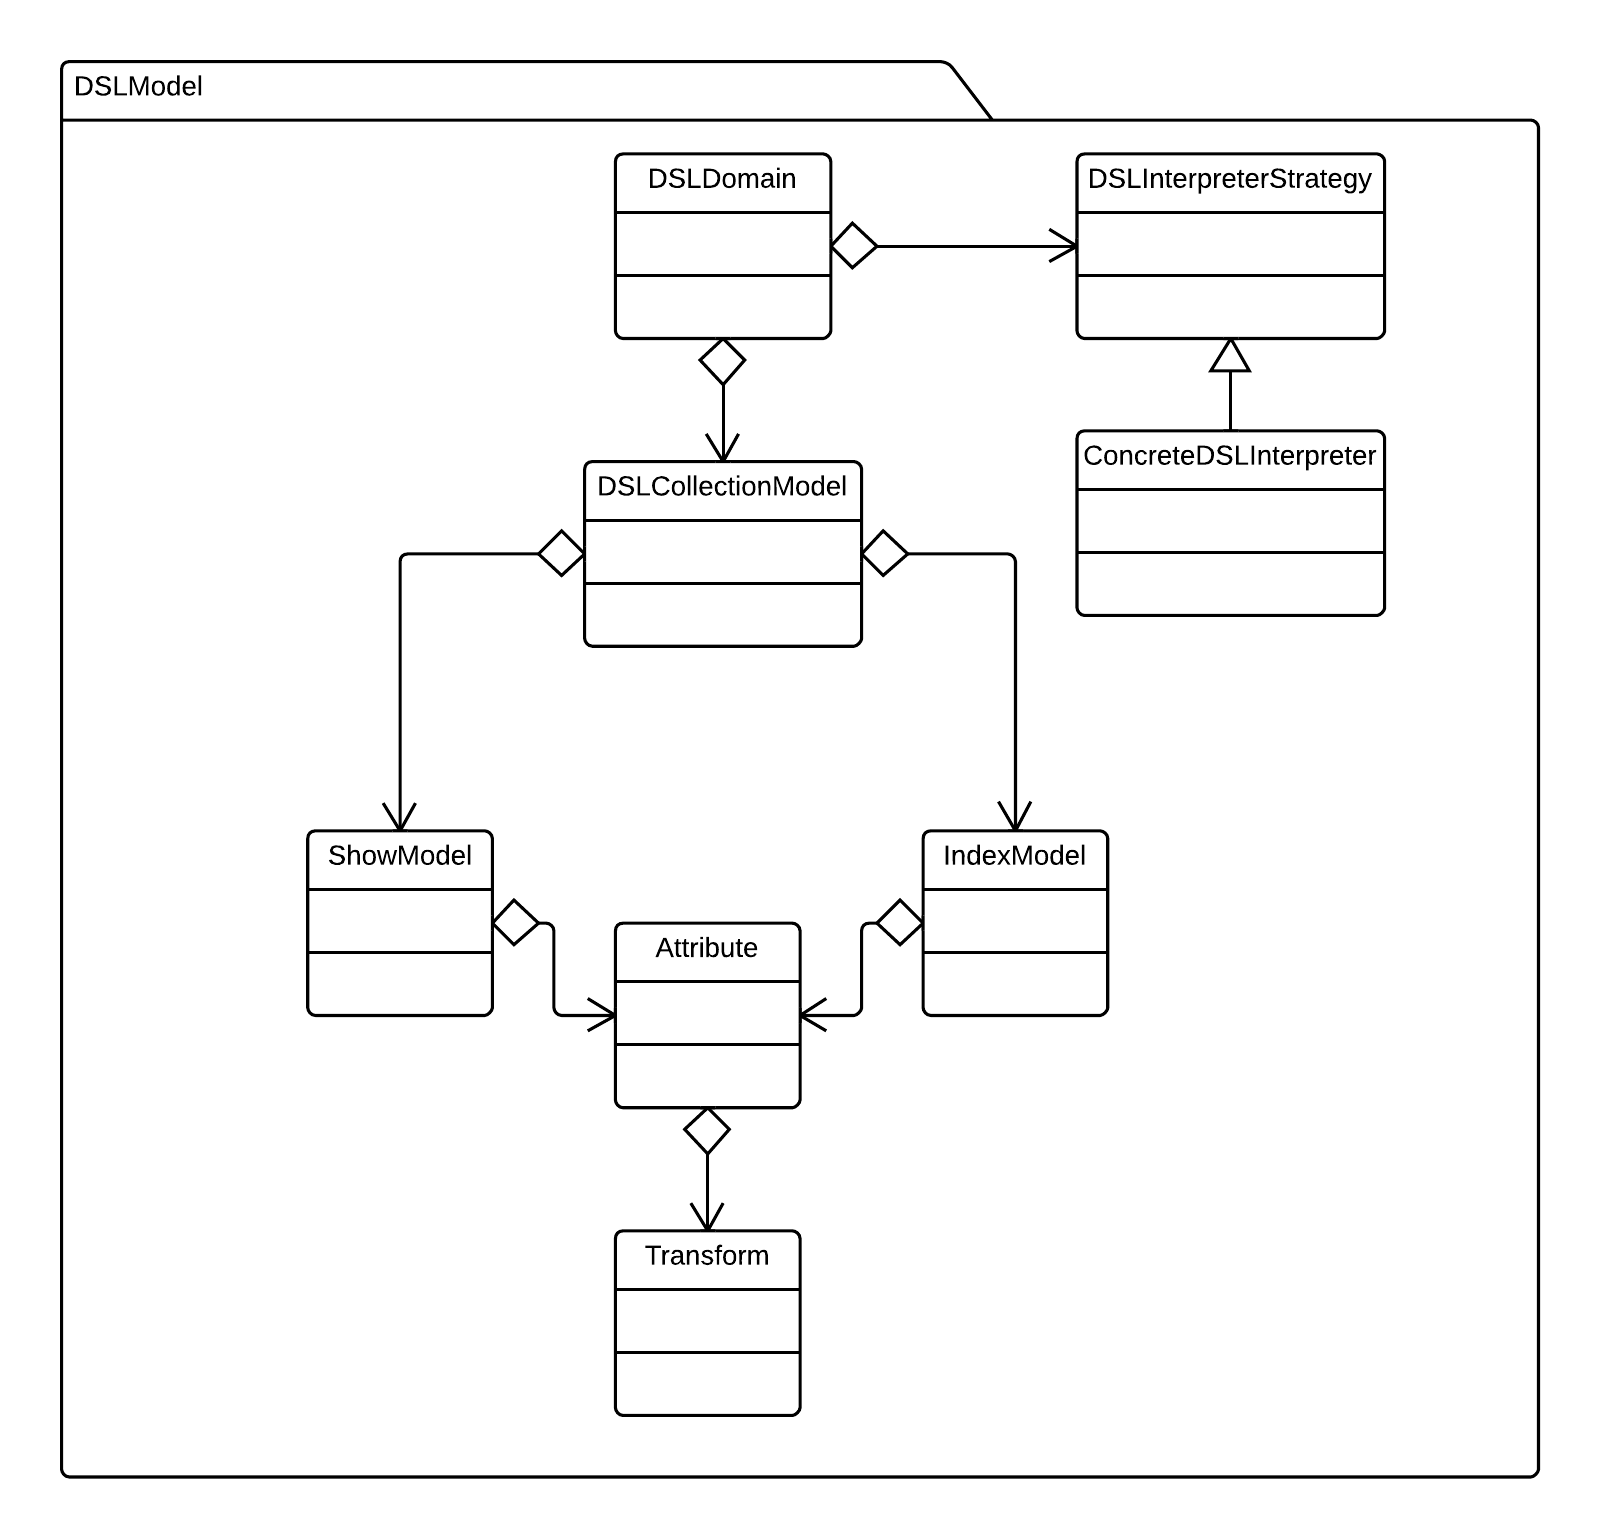
\includegraphics[width=\textwidth]{uml/package/Back-end::Lib::Model::DSLModel.png}  
				\caption{Componente DSLModel}
			\end{center}  
		\end{figure} 
	\subparagraph{Descrizione} 
		\begin{itemize}
		\item[] \glossario{Package} costituito da classi per la definizione delle regole di business sui dati definite tramite il \glossario{DSL} . Il \glossario{package} contiene principalmente classi che si occupano del caricamento del \glossario{DSL} e della sua rappresentazione in un modello ad oggetti. Costituisce la componente model dell’architettura MVC del back-end.

		\end{itemize} 
		\paragraph{Classi}
			\subparagraph{DSLDomain}
				
				\textbf{\\ \\ Descrizione} 
					\begin{itemize}
						\item[] Classe che si occupa di caricare i file \glossario{DSL}. Implementa il \glossario{Design Pattern} \glossario{registry}.
					\end{itemize}      
				\textbf{Utilizzo}  
					\begin{itemize}
						\item[] Viene utilizzata per caricare dinamicamente tutti i \glossario{DSL} a partire dal \glossario{database} che le viene passato.
					\end{itemize}
					\textbf{Relazioni con altre classi}
					\begin{itemize}
							\item{Back-end::Lib::Model::DSLModel::DSLInterpreterStrategy}
							\item{Back-end::Lib::Model::DSLModel::DSLCollectionModel}
					\end{itemize}
			\subparagraph{DSLInterpreterStrategy}
				
				\textbf{\\ \\ Descrizione} 
					\begin{itemize}
						\item[] Classe astratta che definisce l'interfaccia dell'algoritmo di interpretazione del linguaggio \glossario{DSL} utilizzato. È il componente strategy del \glossario{Design Pattern} \glossario{strategy}.
					\end{itemize}      
				\textbf{Utilizzo}  
					\begin{itemize}
						\item[] Viene utilizzata per incapsulare e rendere intercambiabile l'algoritmo di interpretazione del linguaggio \glossario{DSL}. In questo modo, se in futuro vi fosse necessità di cambiare l'algoritmo di interpretazione l'algoritmo può variare indipendentemente dal client che ne farà uso.
					\end{itemize}
					\textbf{Estensioni}
					\begin{itemize}
							\item{Back-end::Lib::Model::DSLModel::DSLInterpreterStrategy::ConcreteDSLInterpreter}
					\end{itemize}
			\subparagraph{DSLCollectionModel}
				
				\textbf{\\ \\ Descrizione} 
					\begin{itemize}
						\item[] Classe che si occupa di definire il model della \glossario{Collection} a partire dal \glossario{DSL}. Si ispira all'\glossario{Abstract Syntax Tree}.
					\end{itemize}      
				\textbf{Utilizzo}  
					\begin{itemize}
						\item[] È l'oggetto risultante dell'interpretazione del \glossario{DSL}. Definisce una rappresentazione interna di una \glossario{Collection}.
					\end{itemize}
					\textbf{Relazioni con altre classi}
					\begin{itemize}
							\item{Back-end::Lib::Model::DSLModel::IndexModel}
							\item{Back-end::Lib::Model::DSLModel::ShowModel}
					\end{itemize}
			\subparagraph{IndexModel}
				
				\textbf{\\ \\ Descrizione} 
					\begin{itemize}
						\item[] Classe che racchiude tutte le informazioni relative ad una index-page. Tali informazioni vengono dichiarate dal developer nel DSL. È composta da un numero variabile di attributi, definiti dalla classe \texttt{Back-end::Lib::DSLModel::Attribute}.
					\end{itemize}      
				\textbf{Utilizzo}  
					\begin{itemize}
						\item[] Questa classe viene creata dalla componente che si occupa di caricare il DSL (interpretandolo o facendone il parsing).
					\end{itemize}
			\subparagraph{ConcreteDSLInterpreter}
				
				\textbf{\\ \\ Descrizione} 
					\begin{itemize}
						\item[] Classe che concretizza l'interprete del \glossario{DSL}. È uno dei componenti ConcreteStrategy del \glossario{Design Pattern} \glossario{Strategy}.
					\end{itemize}      
				\textbf{Utilizzo}  
					\begin{itemize}
						\item[] Viene utilizzata per implementare l'algoritmo utilizzato nell'interfaccia \texttt{Back-end::Lib::DSLModel::DSLInterpreterStrategy} per l'interpretazione del linguaggio \glossario{DSL}. Conterrà al suo interno un metodo che genererà il \glossario{parser} a partire da una grammatica regolare.
					\end{itemize}
					\textbf{Classi Ereditate}
					\begin{itemize}
								\item{Back-end::Lib::Model::DSLModel::DSLInterpreterStrategy}
					\end{itemize}
			\subparagraph{ShowModel}
				
				\textbf{\\ \\ Descrizione} 
					\begin{itemize}
						\item[] Classe che racchiude tutte le informazioni relative ad una show-page. Tali informazioni vengono dichiarate dal developer nel DSL. È composta da un numero variabile di attributi, definiti dalla classe \texttt{Back-end::Lib::DSLModel::Attribute}.
					\end{itemize}      
				\textbf{Utilizzo}  
					\begin{itemize}
						\item[] Questa classe viene creata dalla componente che si occupa di caricare il DSL (interpretandolo o facendone il parsing).
					\end{itemize}
					\textbf{Relazioni con altre classi}
					\begin{itemize}
							\item{Back-end::Lib::Model::DSLModel::Attribute}
					\end{itemize}
			\subparagraph{Trasform}
				
				\textbf{\\ \\ Descrizione} 
					\begin{itemize}
						\item[] Classe che racchiude tutte le informazioni relative alla modalità con cui i dati prelevati dal database verranno modificati prima di essere inviati al front-end.
Tali trasformazioni vengono dichiarate dal developer nel DSL.
					\end{itemize}      
				\textbf{Utilizzo}  
					\begin{itemize}
						\item[] Questa classe viene creata dalla componente che si occupa di caricare il DSL (interpretandolo o facendone il parsing).
					\end{itemize}
			\subparagraph{Attribute}
				
				\textbf{\\ \\ Descrizione} 
					\begin{itemize}
						\item[] Classe che racchiude tutte le informazioni relative ad un attributo di una show-page o di una index-page. Tali informazioni vengono dichiarate dal developer nel DSL.
					\end{itemize}      
				\textbf{Utilizzo}  
					\begin{itemize}
						\item[] Questa classe viene creata dalla componente che si occupa di caricare il DSL (interpretandolo o facendone il parsing).
					\end{itemize}
					\textbf{Relazioni con altre classi}
					\begin{itemize}
							\item{Back-end::Lib::Model::DSLModel::Trasform}
					\end{itemize}
	\subsubsection{Back-end::Lib::Utils}
	\paragraph{Informazioni sul package} 
		\begin{figure}[H] 
			\begin{center} 
				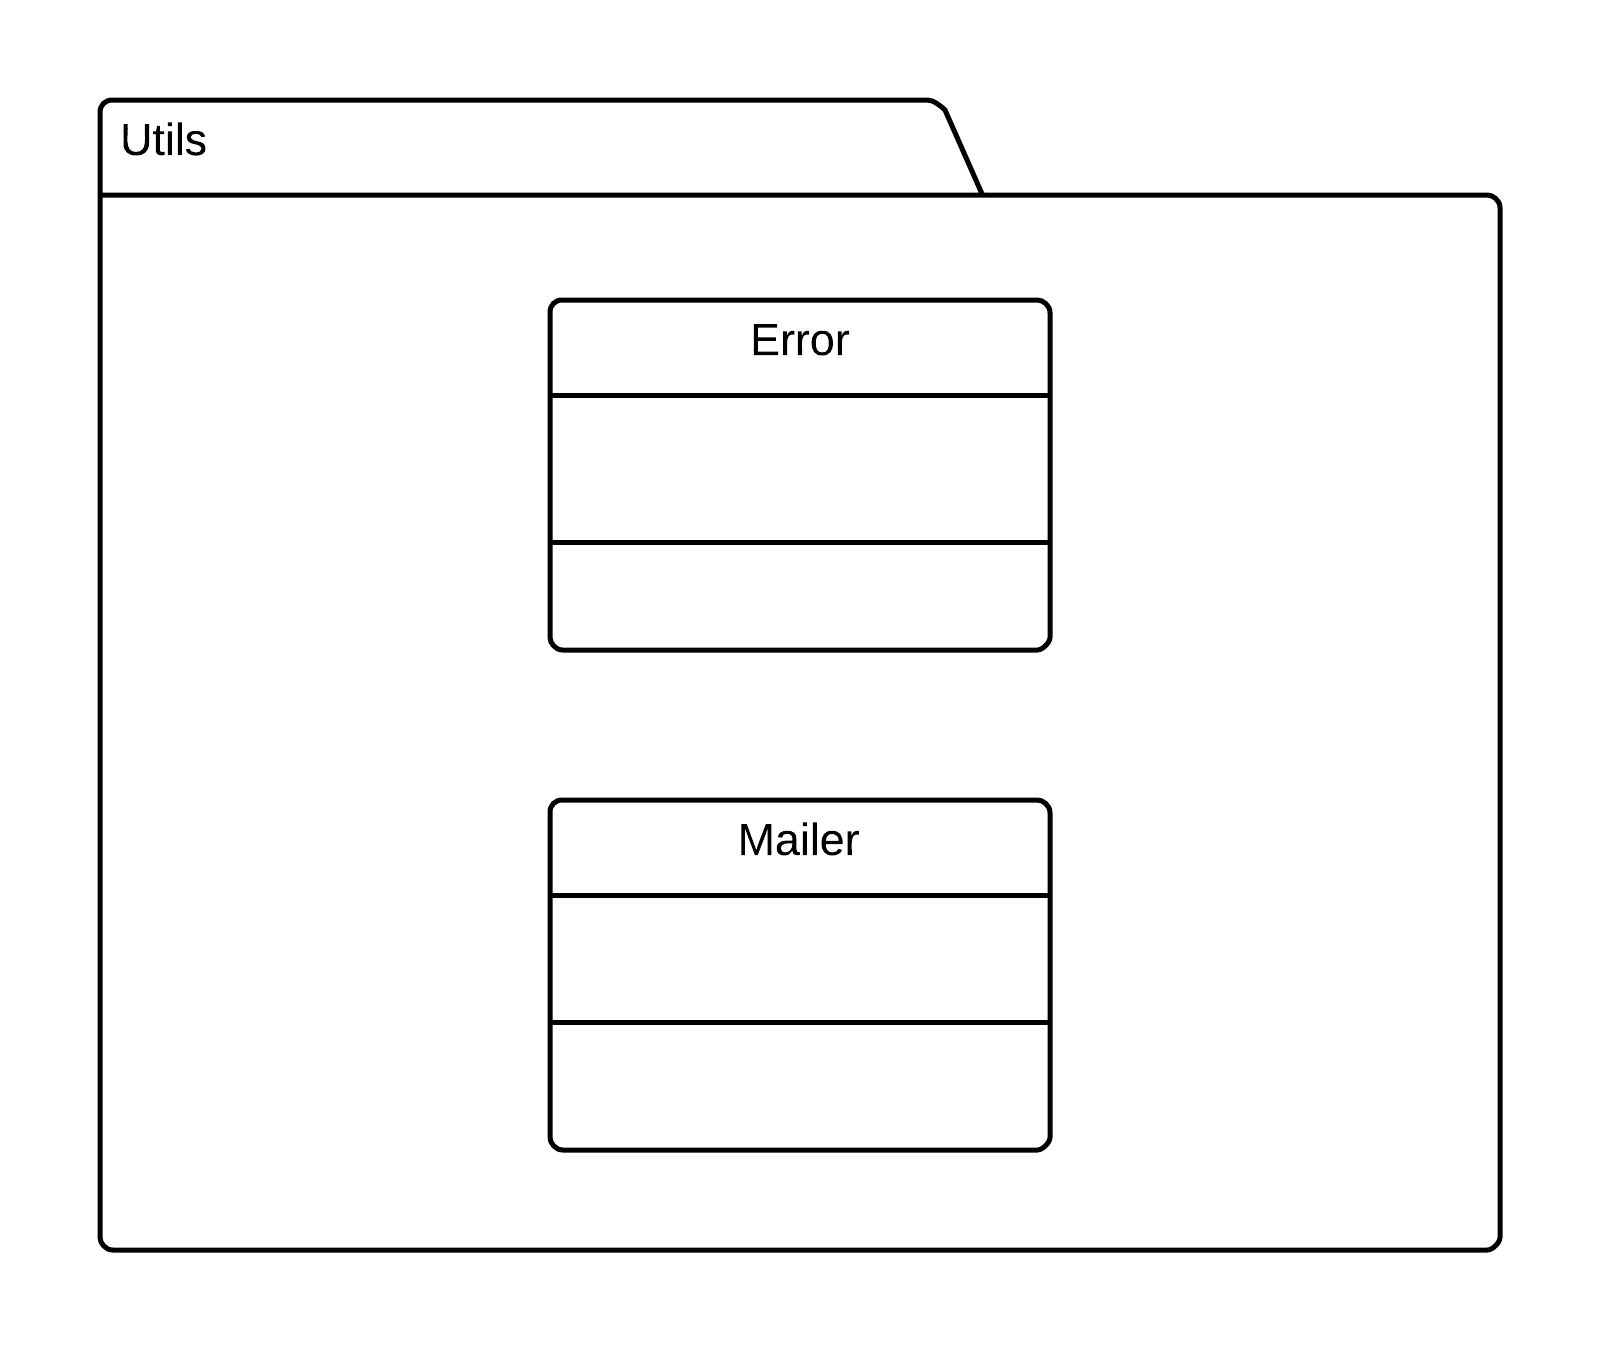
\includegraphics[scale=0.2]{uml/package/Back-end::Lib::Utils.png}  
				\caption{Componente Utils}
			\end{center}  
		\end{figure} 
	\subparagraph{Descrizione} 
		\begin{itemize}
		\item[] \glossario{Package} comprendente le classi di generica utilità, che non rientrano nella classificazione tra model, view e controller.
		\end{itemize} 
		\paragraph{Classi}
			\subparagraph{Mailer}
				
				\textbf{\\ \\ Descrizione} 
					\begin{itemize}
						\item[] Classe che si occupa dell'invio di email. È uno dei componenti subsystem class del \glossario{Design Pattern} \glossario{Facade} e handler del \glossario{Design Pattern} \glossario{Chain of responsibility}.
					\end{itemize}      
				\textbf{Utilizzo}  
					\begin{itemize}
						\item[] Viene utilizzata per inviare un'email ad un utente che ha effettuato la richiesta di recupero password.
					\end{itemize}
			\subparagraph{MaapError}
				
				\textbf{\\ \\ Descrizione} 
					\begin{itemize}
						\item[] Classe che rappresenta un errore all'interno del package \texttt{Back-end::Lib}.
					\end{itemize}      
				\textbf{Utilizzo}  
					\begin{itemize}
						\item[] Viene utilizzata da tutte le classi presente all'interno del package \texttt{Back-end::Lib} per rappresentare un errore generato, identificandolo tramite nome, descrizione e codice.
					\end{itemize}